\documentclass{beamer}
\usepackage[francais]{babel}
\usepackage[utf8]{inputenc}
\usepackage[T1]{fontenc}
\usepackage{graphicx}

\setbeamerfont{page number in head/foot}{}
\setbeamertemplate{footline}[frame number]
\setbeamertemplate{blocks}[shadow=false]

\definecolor{blue1}{rgb}{0.20,0.20,0.70}
\setbeamercolor{block title}{fg=white,bg=blue1}
\setbeamercolor{block body}{fg=black,bg=blue1!10}


\title{Projet de microprocesseur}
\author{Nicolas J., Elie M., Aurélien D. et Louis G.}
\date{28 janvier 2014}

\begin{document}
\maketitle

\section*{Introduction}

\begin{frame}{Vue d'ensemble}
	\begin{figure}
		\centering
		\includegraphics[width=\textwidth,height=0.9\textheight,keepaspectratio]{organisation}
	\end{figure}
\end{frame}

\begin{frame}{Sommaire}
	\tableofcontents
\end{frame}


\section{Simulateur}
% Nicolas et Élie
\begin{frame}{Simulateur - Fonctionnement général}
	\begin{itemize}
		\item Parseur de netlist
		\item Optimizer (ordonne et simplifie les netlists)
		\item Parseur de fichier de ROM
		\item Lecture/Écriture des entrées/sorties du circuit
		\item Initialisation
		\item Cœur du simulateur
	\end{itemize}
\end{frame}
% Décomposé en Optimisation | Utilisation (ROM & entrées/sorties)

\begin{frame}{Simulateur - Fonctionnement interne}
	\begin{block}{Optimizer}
		% Nicolas (TODO)
	\end{block}
	
	\pause
	
	\begin{block}{Simulation}
		\begin{itemize}
			\item Problèmes d'optimisation
			\item Phase d'initialisation pour modifier la structure des données
		\end{itemize}
	\end{block}
\end{frame}

\begin{frame}{Simulateur - Utilisation}
	\begin{block}{ROM}
		\begin{itemize}
			\item Contient le programme à exécuter.
			\item Décrit par un fichier .bin, suite de 0 et 1 pouvant contenir des commentaires.
		\end{itemize}
	\end{block}
	
	\pause
	
	\begin{block}{Entrées/Sorties}
		\begin{itemize}
			\item Utilisations de l'entrée/sortie standard
			\item Communication avec les périphériques par pipe
			\item Possibilité d'asynchronisation de l'entrée
		\end{itemize}
	\end{block}

\end{frame}



\section{Microprocesseur}
% Nicolas et Élie
\begin{frame}{Microprocesseur - Architecture}
	\begin{figure}
		\centering
		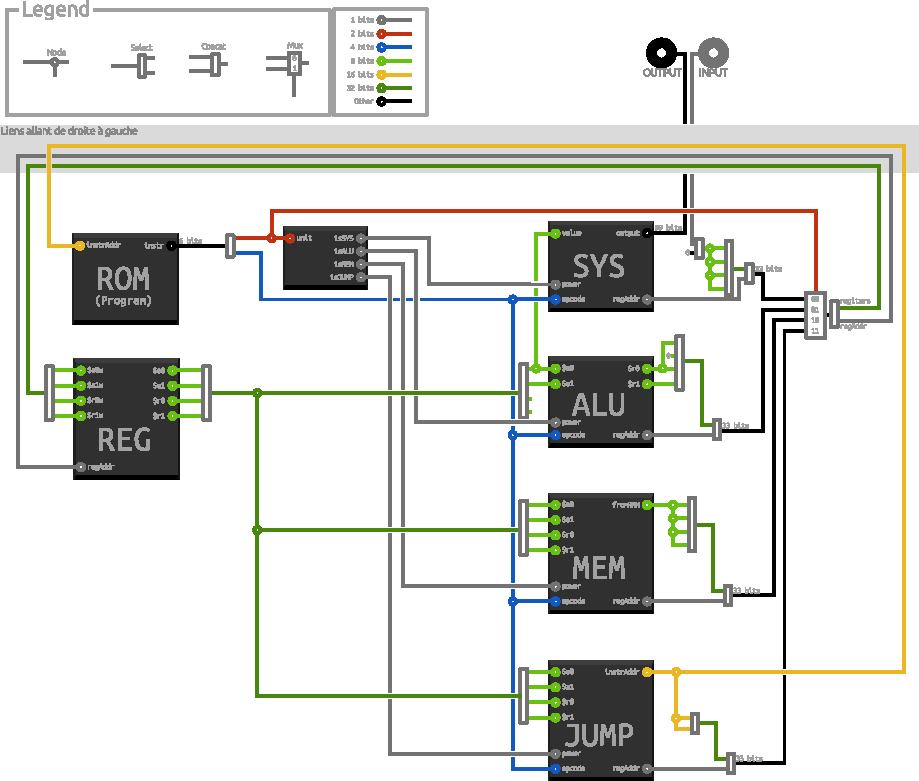
\includegraphics[width=\textwidth,height=0.9\textheight,keepaspectratio]{archi}
	\end{figure}
\end{frame}

\begin{frame}{Microprocesseur - Modification}
	\begin{figure}
		\centering
		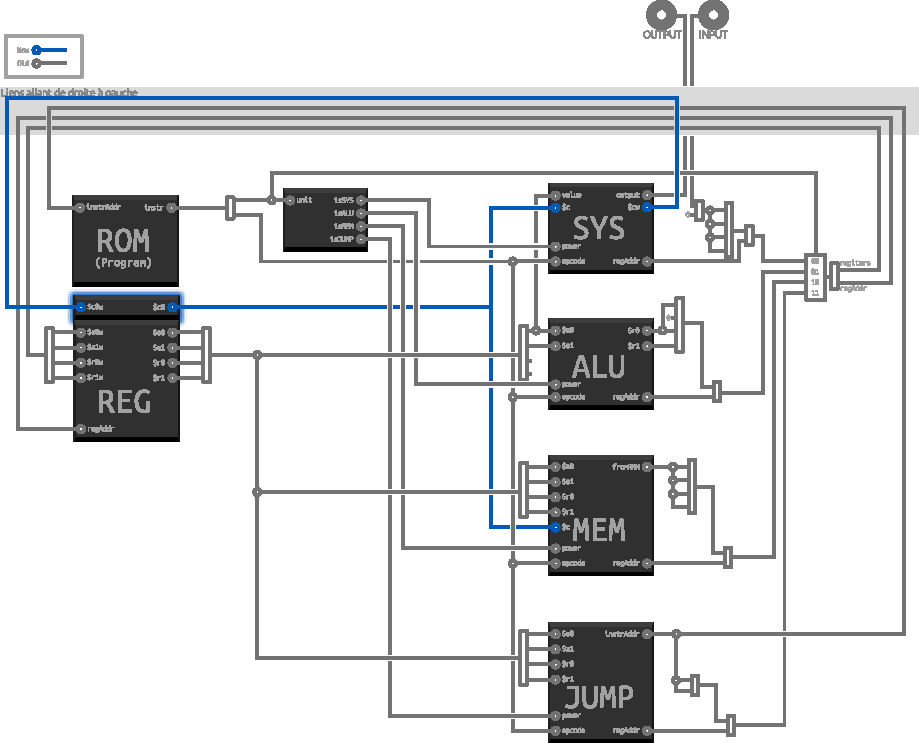
\includegraphics[width=\textwidth,height=0.9\textheight,keepaspectratio]{archi_update}
	\end{figure}
\end{frame}

\begin{frame}{Microprocesseur - Séparation CPU/GPU}
	\begin{figure}
		\centering
		\includegraphics[width=\textwidth,height=0.9\textheight,keepaspectratio]{cpu_gpu}
	\end{figure}
\end{frame}



\section{Programme}
% Louis
\begin{frame}{Programme}
	
\end{frame}


\section{Afficheurs}
% Aurélien
\begin{frame}{Afficheurs}
	
\end{frame}


\section{Oscillateur}
% Élie
\begin{frame}{Oscillateur}
	\begin{figure}
		\centering
		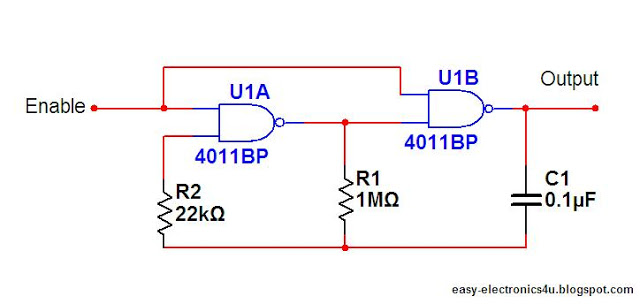
\includegraphics[width=\textwidth,height=0.9\textheight,keepaspectratio]{oscillator.jpg}
	\end{figure}
\end{frame}

\begin{frame}{Oscillateur - Montage}
	\begin{figure}
		\centering
		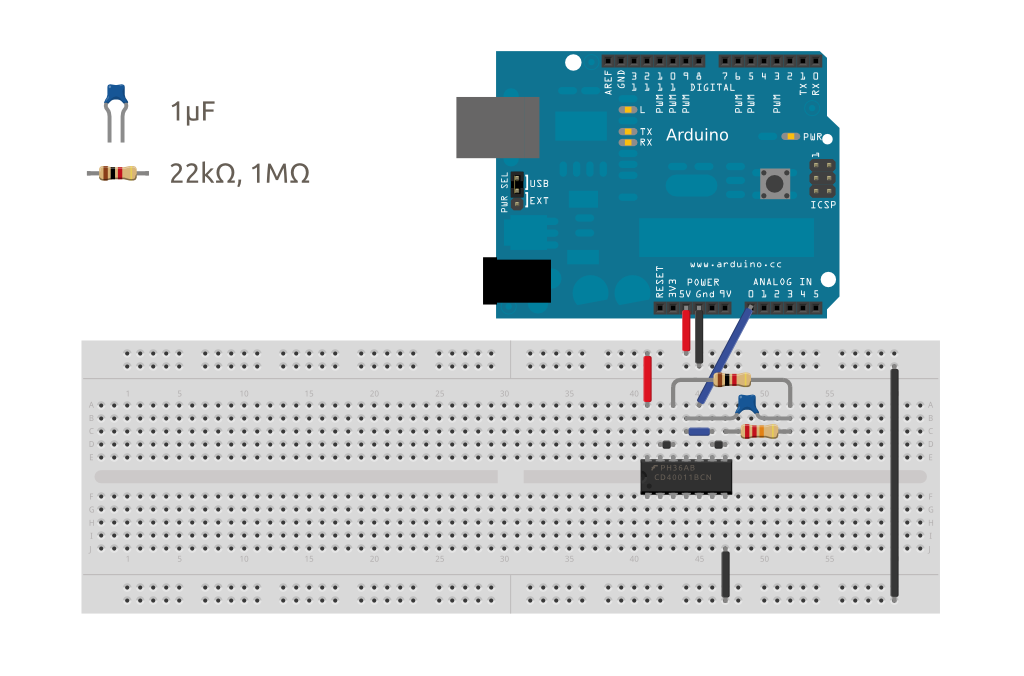
\includegraphics[width=\textwidth,height=0.9\textheight,keepaspectratio]{sysdig_clock}
	\end{figure}
\end{frame}


%<<<<<<<<<<<<<<<<<<<<<<<<<<<<<<<<<<<<<<<< Louis
%\section{Modifications}


%\begin{frame}
%\frametitle{Curseur de lecture}
%\begin{itemize}
%	\item La commande Li ne peut charger directement que de 0 à 7
%	\item Il faut utiliser donc écraser tous les registres pour aller au-delà
%	\item Les adresses mémoire facilement accessibles sont donc seulement de 0 à 7
%	\item On crée donc un pseudo-registre \$c, pour déplacer le curseur de lecture, avec des instructions $incr$ et $decr$
%	\item La RAM comporte non plus 256 mais $2^{16} = 65536$ adresses
%\end{itemize}
%\end{frame}


%\section{Jeu d'instructions}
%\begin{frame}
%\frametitle{Bloc SYS}
%\begin{tabular}{|c|l|l|}
%  \hline
%  Code & Nom & Description \\
%  \hline

%  \hline
%  00 ** ** & \multicolumn{2}{|l|}{SYS} \\
%  \hline
%  00 00 10 & INCR    & Incrémente le curseur de bloc. \\
%  00 00 11 & DECR    & Décrémente le curseur de bloc. \\
%  \hline\hline
%  00 01 00 & INPUT    & \'Ecrit l'input dans un registre donné. \\
%  00 1* ** & OUTPUT x & \'Ecrit \$a0 dans la mémoire graphique\\
%  00 11 11 & FLIP     & Actualise l'affichage du timer \\
%\end{tabular}
%\end{frame}


%\begin{frame}
%\frametitle{Bloc ALU}
%\begin{tabular}{|c|l|l|}
%  \hline
%  00 ** ** & \multicolumn{2}{|l|}{ALU} \\
%	  \hline
%  00 00 ** & \multicolumn{2}{|l|}{Arithmétique} \\
%  \hline
%  01 00 00 & ADD   & \$a0 + \$a1 dans \$r0, retenue dans \$r1 \\
%  01 00 01 & SUB   & \$a1 - \$a0 dans \$r0, retenue dans \$r1 \\
%  01 00 10 & MULT  & \$a0 $*$ \$a1 dans \$r0 . \$r1\\
%  01 00 11 & DIV   & \$a0 = \$r0 $*$ \$a1 + \$r1 \\
%  \hline
%  00 01 ** & \multicolumn{2}{|l|}{Logique} \\
%  \hline
%  01 01 00 & AND   & \$a0 AND \$a1 dans \$r0 (bit à bit) \\
%  01 01 01 & OR    & \$a0 OR \$a1 dans \$r0 (bit à bit) \\
%  01 01 10 & NOT   & \$r0 = NOT( \$a0 ) et \$r1 = NOT( \$a1 ) \\
%  01 01 11 & SHIFT & \$r0 . \$r1 = \$a0 $*$ $2^{\text{\$a1}}$ \\
%  \hline
%  01 1* ** & LI x  & \$a0 = x \\
%	\end{tabular}
%	\end{frame}

%	\begin{frame}
%\frametitle{Bloc MEM}
%\begin{tabular}{|c|l|l|}
%\hline\hline
%  10 ** ** & \multicolumn{2}{|l|}{MEM} \\
%  \hline
%  10 0* ** & \multicolumn{2}{|l|}{entre registres} \\
%  \hline
%  10 00 ij & MOVE 0ij & Déplace un \$a[i] vers un \$r[j]. \\
%  10 01 ij & MOVE 1ij & Déplace un \$r[i] vers un \$a[j]. \\
%  \hline
%  10 1* ** & \multicolumn{2}{|l|}{avec la RAM} \\
%  \hline
%  10 10 ij & LOAD ij  & Charge la valeur en RAM(\$r[i]) dans \$a[j]. \\
%  10 11 ij & SAVE ij  & Enregistre dans RAM(\$r[i]) la valeur \$a[j]. \\
%\end{tabular}
%\end{frame} 

%\begin{frame}
%\frametitle{Bloc JUMP}
%\begin{tabular}{|c|l|l|}
%  \hline\hline
%  11 ** ** & \multicolumn{2}{|l|}{JUMP} \\
%  \hline
%  11 00 ij & JFRA ij & Ajoute \$[i][j] à l'adresse de lecture \\
%  11 01 ij & JBRA ij & Retranche \$[i][j] à l'adresse de lecture \\
%  11 10 ij & IIO  ij & Saute une instruction si le registre donné est $\neq 0$ \\
%  11 11 0i & JAA  i  & Saut à une adresse absolue donnée par \$[i]0.\$[i]1\\
%  11 11 10 & WCA     & \'Ecrit l'adresse courante dans \$a0.\$a1. \\
%  11 11 11 & END      & Termine le programme. \\
%  \hline
%	\end{tabular}
%\end{frame} 

%\section{Programme de l'horloge}


%\begin{frame}
%\frametitle{Mémoire}
%$\overline{\underbrace{\underline{|13|24|29|30|31|32|60|100|}}_{chunk 0}\underbrace{\underline{|j|m|a1|a2|h|mn|s|*|}}_{chunk 1}\underbrace{\underline{|L0|*|L2|*|*|*|*|old|}}_{chunk 2}}$
%\end{frame} 


%\begin{frame}
%\frametitle{Difficultés}
%\begin{itemize}
%	\item Difficile de coder avec si peu d'instructions, mais intéressant
%	\item Surtout lorsqu'il a fallu prendre en compte le nombre de jours par mois
%	\item LUT dans la RAM à l'initialisation
%	\item Réinitialisation de la LUT au changement d'années (pour traiter les années bisextiles)
%	\end{itemize}
%	\end{frame}

%>>>>>>>>>>>>>>>>>>>>>>>>>>>>>>>>>>>>>>>>

\end{document}

